
%Portada del Documento
\chapter{Python}
\setlength{\unitlength}{1 cm} %Especificar unidad de trabajo
\thispagestyle{empty}
\begin{picture}(18,10)
\put(1.5,1){
\includegraphics[width=10cm,height=8cm]{./imagenes4/apli1.png}}
\end{picture}



% fin de la portada


\newpage
\section{ Introducción}

El proyecto realizado con la finalidad de ayudar a personas con discapacidad visual, Interactuando con el usuario por medio de sonido y de instrucciones de voz.
 Consiste en narrar una aventura en la cual nosotros mismos le damos el final dependiendo de las opciones que escojamos,todo esto atravez de instruciones de voz. 
    \subsection{ Requisitos}
\begin{itemize}
\item Instalar Python 2.7.
 \item Instalar la libreria Pygame.
 \item Instalar la libreria Pyaudio.
\item Netbeans 6.9 IDE (no es necesario).
\item Instalar el plugins de Python para netbeans.

\end{itemize}


\begin{figure}[ht!]
 
   \centering
   %%----primera subfigura----
   \subfloat[]{
        \label{fig:pantalla:1}         %% Etiqueta para la primera subfigura
        
\includegraphics[width=0.42\textwidth]{./imagenes4/img1.png}}
   \hspace{0.1\linewidth}
   %%----segunda subfigura----
   \subfloat[]{
        \label{fig:pantalla:2}         %% Etiqueta para la segunda subfigura
        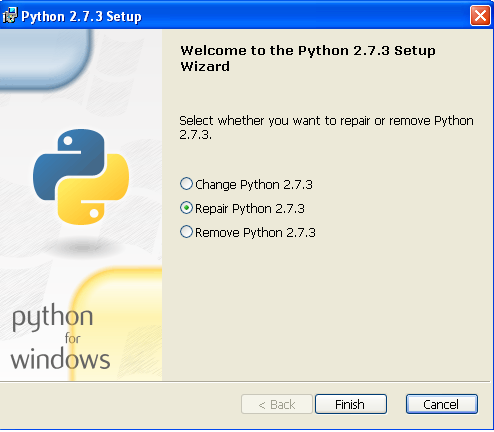
\includegraphics[width=0.42\textwidth]{./imagenes4/img2.png}}\\[20pt]
   %%----tercera subfigura----
   \subfloat[]{
        \label{fig:pantalla:3}         %% Etiqueta para la tercera subfigura
        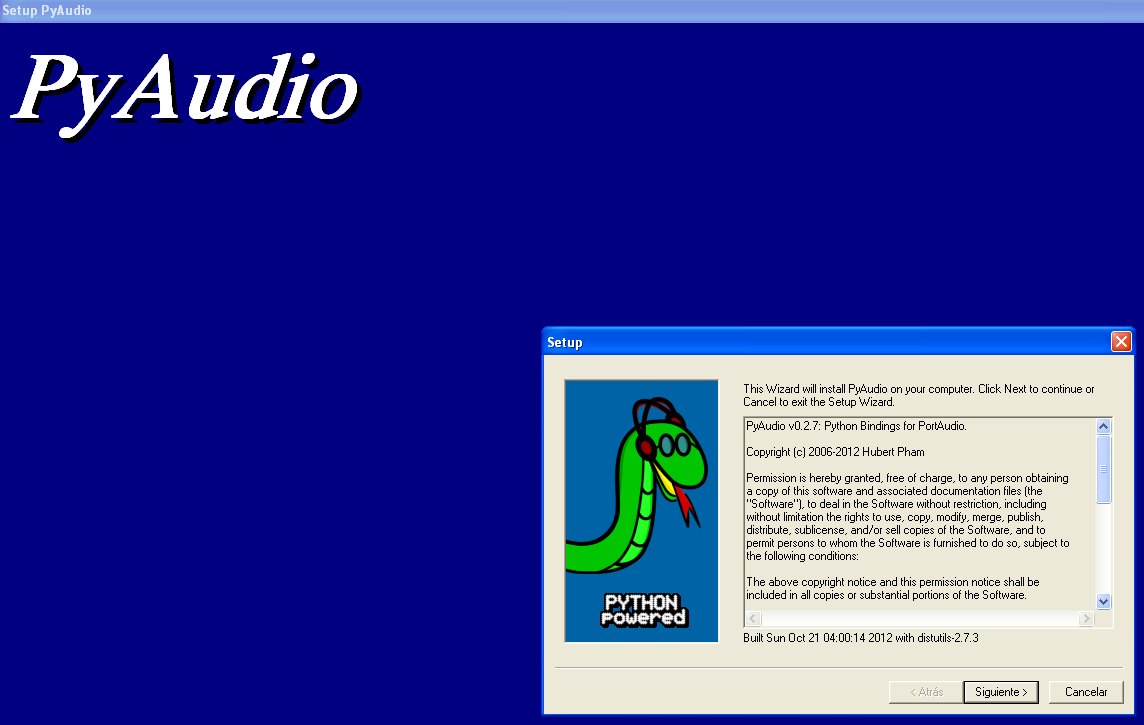
\includegraphics[width=0.42\textwidth]{./imagenes4/dibujo.png}}
\hspace{0.1\linewidth}
 %%----cuarta subfigura----
   \subfloat[]{
        \label{fig:pantalla:4}         %% Etiqueta para la tercera subfigura
        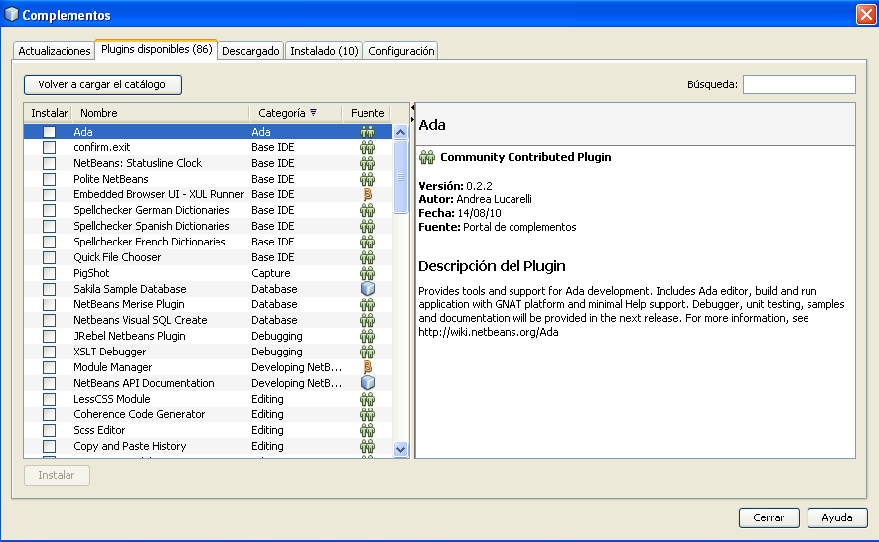
\includegraphics[width=0.42\textwidth]{./imagenes4/img3.png}}
    
\end{figure}


\section{ Como ejecutar el proyecto}
Primero copiamos el archivo del proyecto en cualquier directorio, luego abrimos NetBeans , seguimos los siguientes pasos:
\begin{enumerate}
\item Dar click Archivo -> Abrir Proyecto y buscamos la carpeta del proyecto en el directorio que lo guardamos.
\item Luego en la barra de herramientas dar click en ejecutar.
\end{enumerate}
     
\begin{figure}[ht!]
 
   \centering
   %%----primera subfigura----
   \subfloat[]{
        \label{fig:pantalla:1}         %% Etiqueta para la primera subfigura
        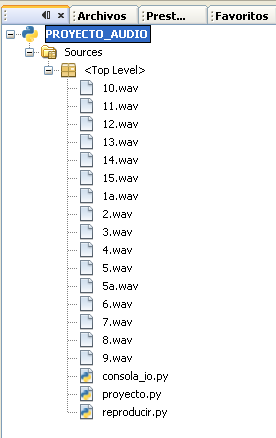
\includegraphics[width=0.42\textwidth]{./imagenes4/img4.png}}
   \hspace{0.1\linewidth}
   %%----segunda subfigura----
   \subfloat[]{
        \label{fig:pantalla:2}         %% Etiqueta para la segunda subfigura
        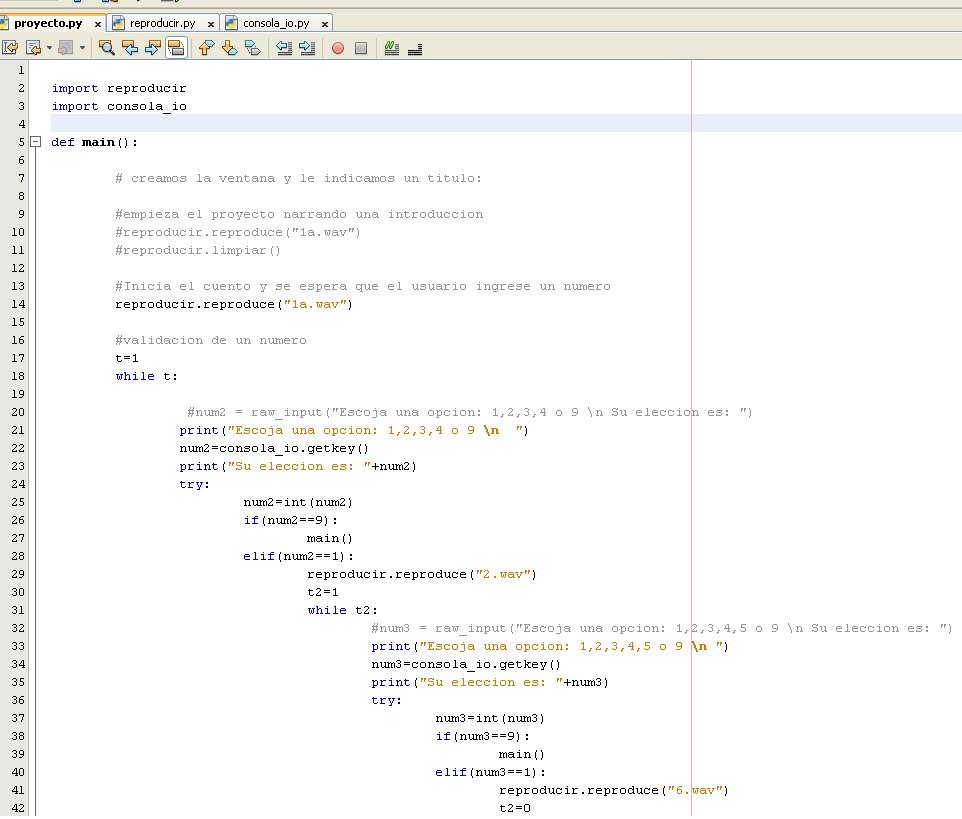
\includegraphics[width=0.42\textwidth]{./imagenes4/img5.png}}
\hspace{0.1\linewidth}
   %%----tercera subfigura----
   \subfloat[]{
        \label{fig:pantalla:3}         %% Etiqueta para la tercera subfigura
        
\includegraphics[width=0.42\textwidth]{./imagenes4/apli.png}}
\end{figure}

\section{ Codigo}
 \begin{verbatim}
   
import reproducir
import consola_io

def main():
        
        # creamos la ventana y le indicamos un titulo:
       
	#empieza el proyecto narrando una introduccion
	#reproducir.reproduce("1a.wav")
	#reproducir.limpiar()

	#Inicia el cuento y se espera que el usuario ingrese un numero
	reproducir.reproduce("1a.wav")

	#validacion de un numero
	t=1
	while t:
               
		 #num2 = raw_input("Escoja una opcion: 1,2,3,4 o 9 \n Su eleccion es: ")
		print("Escoja una opcion: 1,2,3,4 o 9 \n  ")
		num2=consola_io.getkey()
		print("Su eleccion es: "+num2)
		try:
			num2=int(num2)
			if(num2==9):
				main()
			elif(num2==1):
				reproducir.reproduce("2.wav")
				t2=1
				while t2:
					#num3 = raw_input("Escoja una opcion: 1,2,3,4,5 o 9 \n Su eleccion es: ")
					print("Escoja una opcion: 1,2,3,4,5 o 9 \n ")					
					num3=consola_io.getkey()
					print("Su eleccion es: "+num3)
					try:
						num3=int(num3)
						if(num3==9):
							main()
						elif(num3==1):
							reproducir.reproduce("6.wav")
							t2=0
						elif(num3==2):
							reproducir.reproduce("7.wav")
							t2=0
						elif(num3==3):		
							reproducir.reproduce("8.wav")
							t2=0
						elif(num3==4):
							reproducir.reproduce("9.wav")
							t2=0
						elif(num3==5):
							reproducir.reproduce("10.wav")
							t2=0
								
					except ValueError:
						pass
				t=0

			elif(num2==2):
				reproducir.reproduce("3.wav")
				t3=1
				while t3:
					#num4 = raw_input("Escoja una opcion: 1,2 o 9 \n Su eleccion es:  ")
					print("Escoja una opcion: 1,2 o 9 \n ")
					num4=consola_io.getkey()
					print("Su eleccion es: "+num4)
					try:
						num4=int(num4)
						if(num4==9):
							main()
						elif(num4==1):
							reproducir.reproduce("11.wav")
							t3=0
							t4=1
							while t4:
								#num5 = raw_input("Escoja una opcion: 1,2 o 9 \n Su eleccion es: ")
								print("Escoja una opcion: 1,2 o 9 \n ")
								num5=consola_io.getkey()
								print("Su eleccion es: "+num5)
								try:
									num5=int(num5)
									if(num5==9):
										main()
									elif(num5==1):
										reproducir.reproduce("12.wav")
										t4=0
									elif(num5==2):
										reproducir.reproduce("13.wav")
										t4=0
										t5=1
										while t5:
											#num6 = raw_input("Escoja una opcion: 1,2 o 9 \n Su eleccion es: ")
											print("Escoja una opcion: 1,2 o 9 \n ")
											num6=consola_io.getkey()
											print("Su eleccion es: "+num6)
											try:
												num6=int(num6)
												if(num6==9):
													main()
												elif(num6==1):
													reproducir.reproduce("14.wav")
													t5=0
												elif(num6==2):
													reproducir.reproduce("15.wav")
													t5=0
											except ValueError:
												pass


								except ValueError:
									pass


						elif(num4==2):
							reproducir.reproduce("7.wav")
							t3=0
					except ValueError:
						pass
				t=0
				
			elif(num2==3):
				reproducir.reproduce("4.wav")
				t=0
			elif(num2==4):		
				reproducir.reproduce("5.wav")
				main()
		
		except ValueError:
			pass
	print "\nY asi \ncolorin colorado \neste cuento se ha acabado"

#ejemplo limpiar pantalla: reproducir:limpiar 
if __name__ == "__main__":
            main()
 \end{verbatim}

\section{ Experiencias}
\begin{itemize}
\item Python fue un lenguaje nuevo para mi pero debido a toda la informaciòn que hay en internet y a los ejemplos que encontre se me hizo facil. 
\item Solo se uso la libreria de audio para trabajar el proyecto el cual fue divertido realizarlo.  
\item Buscar el libro y grabar la historia fue interesante, tuve que leer muchas historias para ver cual era la mejor para el proyecto.
\item Hubo una historia a que me gusto mucho que se llama " El Misterio de las Piedras Sagradas ", esta historia es muy interesante pero a mi compañero le parecio muy larga asi que tuvimos que buscar otra.
\item La historia que grabamos la encontro mi compañero de proyecto en internet, es divertida y no muy laraga por eso decidimos hacer esa.
   
\end{itemize}


